

\chapter{\uppercase{Experimental Setup and Results}}

The experimental setup consists of a server chassis provided by Viking Technologies \ref{cite:Viking_webpage} with the following configuration. 


\begin{table}[H]
\centering
\caption{Setup Machine Configuration}
\label{tab:unixcomp}
\begin{tabular}{|c|c|c|}
    \hline
    Component & Specification & Quantity \\
    \hline
    \hline
    CPU & E5-2640 & 2                    \\
    \hline
    Motherboard & X9DRH-iF Ver 1.02 & 1  \\
    \hline
    RAM & DDR3 RDIMM & 1 x 4GB           \\
    \hline
    NVRAM & DDR3 ArxCis NVDIMM & 2 x 4GB \\
    \hline
    SSD & SATADIMM & 100GB               \\
    \hline
    OS & Fedora 17 (x86\_64) & -         \\
    \hline
    Kernel & 3.5.1 & -                   \\
    \hline
    Hypervisor & Xen 4.1.5 & -           \\
    \hline
    NVRAM SDK & ArxSDK 1.3 & -           \\
    \hline
\end{tabular}
\end{table}

The BIOS present on this machine marks the NVRAM area with a code of 90 and it occupies the address space from 6GB to 14GB. The software development kit ArxSDK 1.3 provided by Viking Technologies, was used for testing the read/write speeds and operation of NVRAM region.

Mainly two components of the ArxSDK was used for profiling purposes.

1. Driver: The driver code programs the Integrated Memory Controller to query for the presence of NVDIMMs. It stores relevant information such as the start address, size and number of NVDIMMs, allowing a host of ioctl commands for additional programming of the IMC.

2. Test Code: This code obtains the available NVRAM physical address space from the driver, and maps the former to its own address space using the mmap system call. It proceeds to write data sequentially to this region and read it back. It reports the amount of time taken to complete the whole test as a rough measure of throughput.

The driver code was modified to remove most of the above mentioned functionality, since access to the IMC and other privilege commands are not available to a guest domain. Performance measurements were taken using the perf profiling tool, but without any significant advantage. The perf tool collects hardware performance counters such as TLB misses, L1 cache misses, L2 cache misses, etc., but these measurements are not available in a guest domain in Xen.

Each guest domain is equipped with 3.5GB of non-volatile RAM for this test with the cache set to Write Back mode. The results presented in Fig~\ref{fig:result_fig} compares three cases

1. Test running on 1 guest domain.

2. Tests running on 2 guest domains simultaneously.

3. Test running on the bare Linux (the same version 3.5.1) without the hypervisor.

One run of the test code writes a predetermined sequence to the whole 3.5GB non-volatile memory area, and then reads it back. This code is run five times and the CPU time taken in the whole procedure is recorded as a single reading. Each case is tested multiple times (>14 times), and a very low standard deviation is observed in the results as indicated by the error bars. 


\begin{figure}[H]
\centering
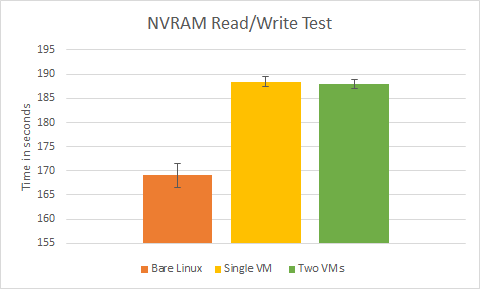
\includegraphics{figures/read_write_test.png}
\caption{Comparison of Read/Write performance of Bare Linux vs Single VM and vs Two VMs}
\label{fig:result_fig}
\end{figure}



In the graph present above, it can be observed that there is a visible overhead (~12\% as compared to bare Linux case) for operating in a virtualized environment. However, there is hardly any difference observed between the cases of running a single VM versus that of running two VMs. This can be explained by the fact that system time in a virtual environment is quite different from the wall clock time. For a guest domain, the vCPU time increases only as long as the guest domain occupies that resource. When it is swapped for another virtual machine, the vCPU clock corresponding to the domain is stopped. Thus from the perspective of a virtual machine, the performance should remain similar irrespective of the number of VMs running on the machine. The higher time cost observed in a virtual environment as compared to a bare Linux can be attributed to a combination of hardware and software factors such as higher penalty for TLB misses and overhead for operating on top of Xen.

Several screenshots are attached below which present various stages of the NVM sharing. Fig ~\ref{fig:xen_boot} displays part of the original E820 Memory Map generated by the BIOS and received by Xen. The whole list is quite long supporting numerous reserved regions for MMIO

devices. In the last line, NVRAM, indicated with code 90, can be seen occupying the address space from 6GB to 14GB. 

\begin{figure}[H]
\centering
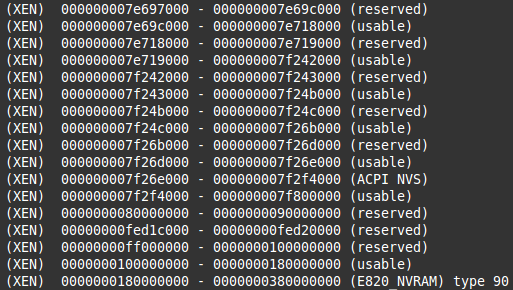
\includegraphics{figures/xen_e820.png}
\caption{Machine E820 memory map}
\label{fig:xen_boot}
\end{figure}

Fig ~\ref{fig:bochs} shows the Xen kernel level logging messages on the creation of a domU with the 892MB of RAM and 3.5GB of NVRAM. The virtual E820 layout generated by Bochs code shows the various regions, with holes introduced for I/O devices. NVRAM is mapped from 4GB to 7.5GB, in consideration with the Arxcis SDK 1.3 which requires the non-volatile memory to be placed above 4GB in aligned blocks of 512MB. This proves beneficial in several ways

1. A separate driver need not be developed, allowing reuse of existing framework.

2. Several Linux kernel versions change the unrecognized code 90 (or 0x5A in hexadecimal) in the E820 table to code 2, marking it as an I/O space, thereby making NVRAM discovery process extremely difficult. This ordeal can be avoided altogether by placing the non-volatile memory above 4GB, since, chipsets typically place I/O devices just below the 4GB mark. Therefore, any I/O region found above 4GB can be assumed to be non-volatile memory.

3. Aligning the NVM region on the gigabyte boundary and placing it above 4GB (avoiding the virtual MMIO hole introduced by Bochs), reduces the fragmentation of the NVRAM address space. This allows for superpage allocations of 1GB pages in the hypervisor page tables, reducing the total number of page table entries and potential TLB misses. 

\begin{figure}[H]
\centering
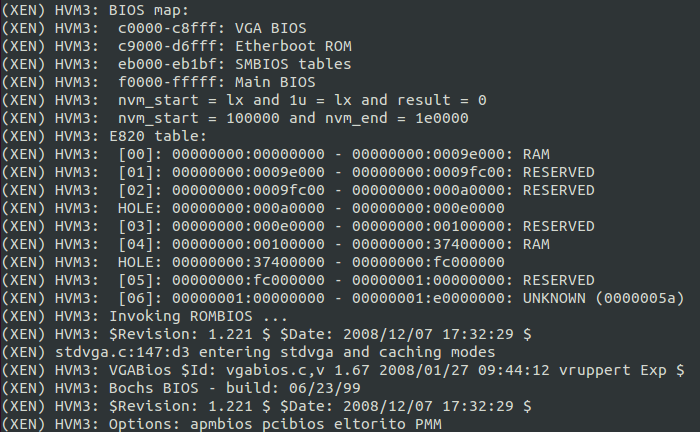
\includegraphics[scale=0.8]{figures/domu_boot1.png}
\caption{DomU boot up kernel messages}
\label{fig:bochs}
\end{figure}

The actual page allocation is visible in the figure below. Since the RAM address space is fragmented, it contains a combination of 2MB and 4KB pages to satisfy its request. However, NVRAM occupies a contiguous address space comprising of three, 1GB pages and 256, 2MB pages. 


\begin{figure}[H]
\centering
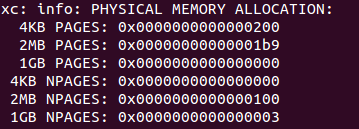
\includegraphics{figures/page_allocation_domu.png}
\caption{DomU page allocation}
\label{fig:page_alloc}
\end{figure}


